\documentclass[12pt,a4paper]{book}
\usepackage{fontspec}         
\setmainfont{Arial}
\newfontfamily{\cyrillicfonttt}{Arial}
\newfontfamily{\cyrillicfont}{Arial}
\newfontfamily{\cyrillicfontsf}{Arial}
\usepackage{polyglossia}     
\setdefaultlanguage{russian}  
\setotherlanguage{english}
\usepackage{fancyhdr} % Колонтитулы
\pagestyle{fancy}
\usepackage{float}
\usepackage{hyperref}
\hypersetup{
    unicode=true,           % позволяет использовать юникодные символы
    colorlinks=true,       	% true - цветные ссылки, false - ссылки в рамках
    urlcolor=black,          % цвет ссылки на url
    linkcolor=black,          % внутренние ссылки
    citecolor=green,        % на библиографию
	pdfnewwindow=true,      % при щелчке в pdf на ссылку откроется новый pdf
	breaklinks              % если ссылка не умещается в одну строку, разбивать ли ее на две части?
}
\usepackage[paper=a4paper,top=10mm, bottom=10mm,left=35mm,right=35mm,includefoot,includehead]{geometry}
\setlength{\parskip}{4mm}
\newcommand{\mysize}[2]  
{{\fontsize{#1}{1}\selectfont #2 }}
\usepackage{graphicx}                 
\usepackage{graphics}
\usepackage{afterpage}

\newcommand{\newsize}[1]  
{{\fontsize{14}{1}\selectfont #1 }}
\renewcommand{\headrulewidth}{0.2pt}


\usepackage{fancyhdr} 
\pagestyle{fancy}
\setcounter{page}{3}
\renewcommand{\thesection}{Приложение \Asbuk{section}}
\setcounter{section}{0}

\renewcommand{\headrulewidth}{0.2pt} 

\lfoot{}
\rfoot{}
\rhead{\thepage}

\lhead{\rightmark}
\cfoot{Школа Чародейства и Волшебства "Хогвартс"}




\renewcommand{\labelitemi}{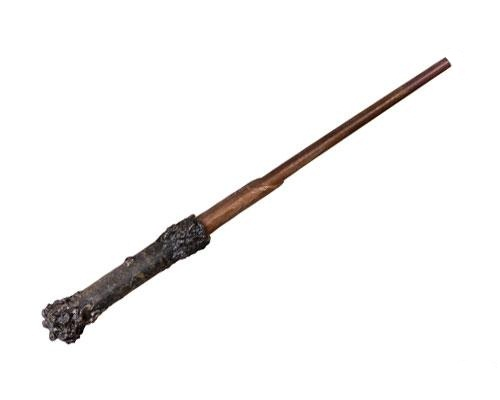
\includegraphics[height=8mm]{magic.jpg}}
\flushbottom                            
\righthyphenmin=6
 
\begin{document}
 
 \begin{titlepage}
 \thispagestyle{empty}
 
\setlength{\parindent}{0cm}

 \begin{figure} [H]
  \begin{center}
  
 
\includegraphics[height=6cm]{emblem.jpg}
 \end{center}
 \end{figure}
 \vspace{1cm}

 
 Мисс Шери
 
 \vspace{2cm}
 \newsize{Дорогая Мисс Шери,\\
 
 Мы рады проинформировать Вас, что Вам представлено\\
 место в школе Чародейства и Волшебства  ''Хогвартс''.\\
 
 Пожалуйста, ознакомьтесь с приложенным к данному письму списком необходимых книг и предметов.\\
 
 Занятия начинаются 1~сентября. Ждем Вашу сову не позднее 31~июля.\\
 
 Искренне Ваша,\\
 

 {\Huge{\fontspec{DearMrPotter}{Minerva}}}\\
 Минерва МакГонагалл\\
 
 заместитель директора 
 
 \vspace{\fill}
 \begin{center}
\href{https://github.com/bdemeshev}{Школа Чародейства и Волшебства ''Хогвартс''}\\
 \normalsize{ Директор: Альбус Дамблдор\\
 (Кавалер ордена Мерлина первой степени,\\ основатель Ордена
 Феникса, \\председатель Международной Конфедерации Магов }
 \end{center}
 }

\end{titlepage}

\newpage

\section {Список необходимых книг и предметов}
\begin{itemize}
\item Волшебная палочка
\item Мантия-невидимка
\item Камень, оживляющий мёртвых
\item Задачник Демидовича 
\end{itemize}

\newpage

\section {Cписок изучаемых предметов}

\begin{itemize}
\item Трансфигурация
\item  История магии
\item Математический анализ

\end{itemize}

\end{document}